% Provenance (never printed): old seconde/premiere S material on soil as a
% slowly renewed resource (alteration of rocks, clays, the clay--humus
% complex, soil erosion); see sources/book2/PROVENANCE.md. Rates are the
% medians of Montgomery (2007), computed in figdata/grade-10/soil_rates.py.
\chapter{Soil, a Slow-Forming Resource}\label{ch:g10:soil-formation}

A road cut through a hillside in the humid tropics shows a wall of red
earth, several times the height of a person. At its foot the rock is still
recognisable: pale, streaked, but so soft that it crumbles between the
fingers while still showing the grains and bands of the rock it once was.
Upwards it turns into a mottled clay, then into a hard red layer, then into a
thin soil where the roots are. The whole wall was once solid rock: it is the
rock itself, slowly transformed in place by water and air. Soil, on which all
the land's plants and the food of almost all people grow, is the top of such
a column. This chapter explains how rock becomes soil, what chemistry does
the work, how climate sets its pace, and why soil, so slow to form, can be
lost so quickly.

\begin{omfigure}
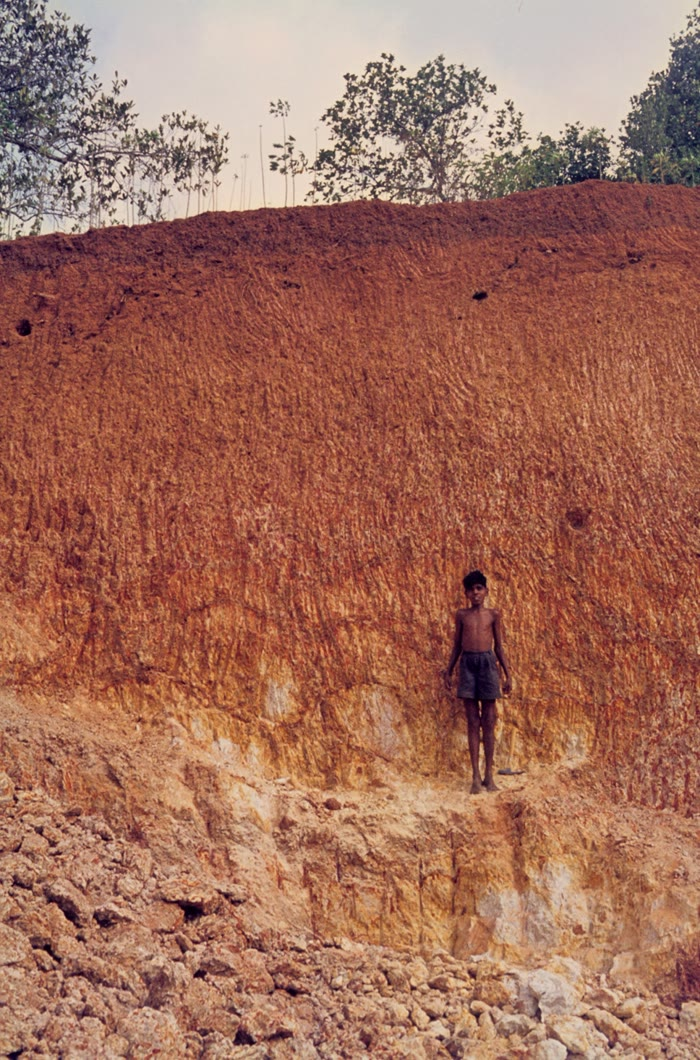
\includegraphics[height=8.5cm]{images/book2/g10-laterite-kerala.jpg}

{\small A weathering profile on granitic gneiss in Kerala, southern India: at
the bottom, a mottled, decomposed rock; above, a brown, weakly hardened
\omterm{def:g10:soil-formation:laterite}{laterite} under a thin soil. The boy gives the scale. Photograph: Werner
Schellmann, 1969 (CC~BY-SA~2.5).}
\end{omfigure}

\begin{recall}
Weathering breaks rocks down where they lie; erosion carries the pieces
away; deposition lays them down elsewhere (Book 1, grade 5). Rocks are made
of minerals, such as quartz, feldspars and micas in a granite (Book 1, grade
6). A soil is a living layer of mineral grains, humus, water, air and
organisms; decomposers turn dead matter into humus; a soil is described by
its layers, or horizons (the biology books). In an oxidation, a substance
loses electrons, often by combining with oxygen (the chemistry books).
\end{recall}

\section{From rock to soil}

Physical weathering --- frost wedging, heating and cooling, roots ---
breaks rock into pieces without changing its minerals. \omterm{def:g10:soil-formation:chemical-weathering}{Chemical weathering}
changes the minerals themselves. Together, over long times, they turn the top
of the solid rock into a loose mantle that thickens downwards as weathering
eats into the rock below.

\begin{definition}[Parent rock; saprolite]\label{def:g10:soil-formation:weathering-profile}
The \emph{parent rock}\index{parent rock} of a soil is the rock from which its
mineral part was formed. \emph{Saprolite}\index{saprolite} is rock decomposed
in place by weathering: soft and earthy, it still shows the grains and the
structure of the parent rock. A \emph{weathering profile} is the whole column
from the fresh rock, through the saprolite, to the soil at the top.
\end{definition}
% ledger: usgs:saprolite

\omterm{def:g10:soil-formation:weathering-profile}{Saprolite} can be thick. Under the rolling hills along the eastern side of the
Appalachian Mountains, in the eastern United States, it reaches about
\qty{46}{m} (150 feet) in places, though its thickness varies a great deal
from place to place; the soil is only the upper part of it.
% ledger: usgs:saprolite

\begin{omfigure}
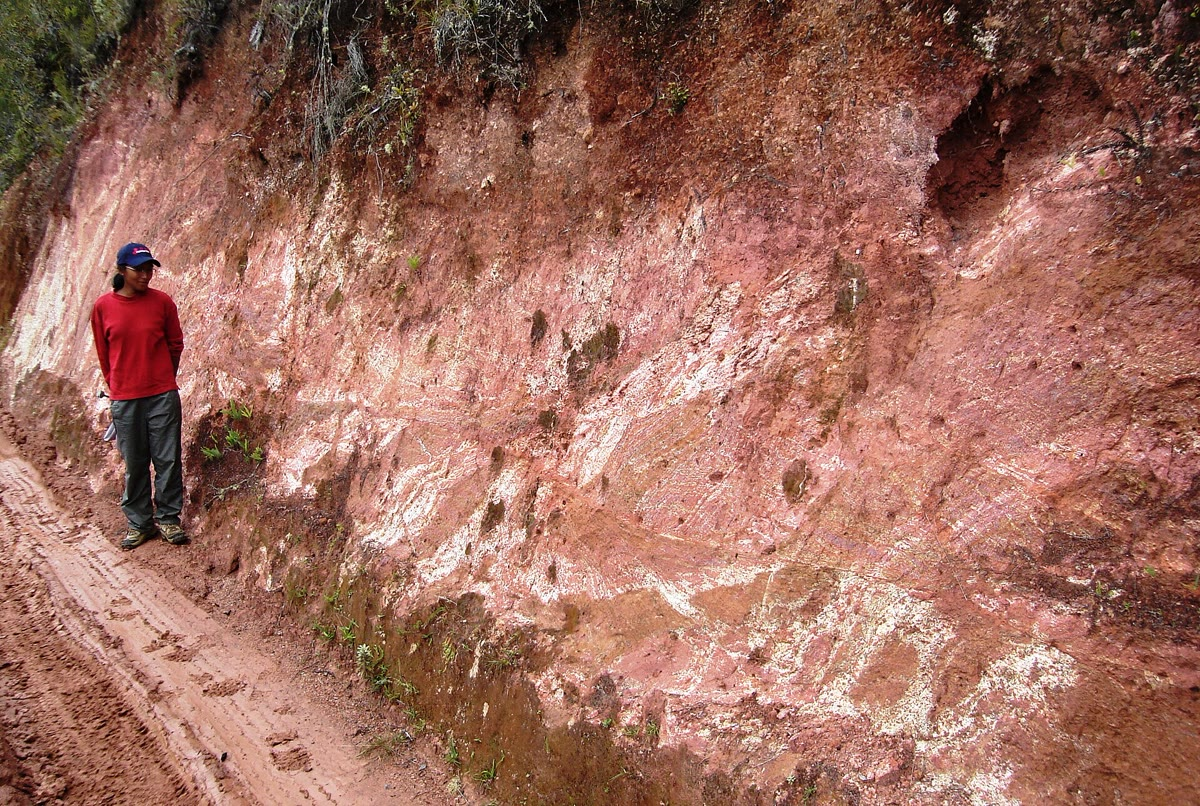
\includegraphics[width=0.8\linewidth]{images/book2/g10-saprolite-madagascar.jpg}

{\small \omterm{def:g10:soil-formation:weathering-profile}{Saprolite} in a road cut in central Madagascar: the old gneiss,
decomposed in place, still shows its bands as streaks of white clay in red
earth. Photograph: Diorit (CC~BY-SA~3.0).}
\end{omfigure}

\begin{omfigure}
\begin{tikzpicture}[font=\footnotesize]
  % humid tropical column
  \begin{scope}
    \fill[omThm!45!brown!60] (0,5.4) rectangle (1.8,6.0);
    \fill[omThm!70!orange!70] (0,4.2) rectangle (1.8,5.4);
    \fill[omThm!25!orange!35] (0,1.2) rectangle (1.8,4.2);
    \foreach \y in {1.5,2.1,2.7,3.3,3.9} \draw[white!80!black, thick] (0.1,\y) -- (1.7,\y+0.15);
    \fill[black!30] (0,0) rectangle (1.8,1.2);
    \foreach \x/\y in {0.3/0.3,0.9/0.7,1.4/0.2,0.5/0.9,1.2/1.0} \draw[black!55] (\x,\y) -- ++(0.2,0.08);
    \draw[black!60] (0,0) rectangle (1.8,6.0);
    \node[anchor=north, align=center] at (0.9,-0.1) {humid tropics};
  \end{scope}
  % temperate column
  \begin{scope}[xshift=3.2cm]
    \fill[omThm!45!brown!60] (0,2.2) rectangle (1.8,2.6);
    \fill[omThm!25!orange!35] (0,1.2) rectangle (1.8,2.2);
    \foreach \y in {1.5,1.9} \draw[white!80!black, thick] (0.1,\y) -- (1.7,\y+0.15);
    \fill[black!30] (0,0) rectangle (1.8,1.2);
    \foreach \x/\y in {0.3/0.3,0.9/0.7,1.4/0.2,0.5/0.9,1.2/1.0} \draw[black!55] (\x,\y) -- ++(0.2,0.08);
    \draw[black!60] (0,0) rectangle (1.8,2.6);
    \node[anchor=north, align=center] at (0.9,-0.1) {temperate\\climate};
  \end{scope}
  % labels
  \draw[black!50] (5.3,5.7) -- (2.0,5.7); \node[anchor=west] at (5.4,5.7) {soil};
  \draw[black!50] (5.3,4.8) -- (2.0,4.8); \node[anchor=west, align=left] at (5.4,4.8) {laterite: red, rich in iron\\and aluminium oxides};
  \draw[black!50] (5.3,3.4) -- (2.0,3.4); \node[anchor=west, align=left] at (5.4,3.4) {saprolite: rock decomposed\\in place, structure kept};
  \draw[black!50] (5.3,0.6) -- (5.0,0.6); \node[anchor=west] at (5.4,0.6) {fresh parent rock};
\end{tikzpicture}

{\small Two weathering profiles on the same rock (schematic, not to scale):
under a hot, wet climate the profile is much thicker and its top is a
\omterm{def:g10:soil-formation:laterite}{laterite}; under a temperate climate a thinner \omterm{def:g10:soil-formation:weathering-profile}{saprolite} carries the soil.}
\end{omfigure}

\section{Chemical weathering}

\begin{definition}[Chemical weathering]\label{def:g10:soil-formation:chemical-weathering}
\emph{Chemical weathering}\index{chemical weathering} is the transformation
of the minerals of a rock by reactions with water and with the gases it
carries, carbon dioxide and oxygen: some minerals dissolve, others are turned
into new minerals, stable at the Earth's surface.
\end{definition}

Rainwater dissolves a little carbon dioxide from the air, and much more as it
seeps through the soil, where roots and decomposers breathe it out. Part of
the dissolved gas forms carbonic acid, which releases hydrogen ions:
\begin{center}
\ce{CO2 + H2O -> H+ + HCO3-}
\end{center}
These hydrogen ions attack the minerals.

\begin{definition}[Hydrolysis]\label{def:g10:soil-formation:hydrolysis}
\emph{Hydrolysis}\index{hydrolysis} is the \omterm{def:g10:soil-formation:chemical-weathering}{chemical weathering} of a silicate
mineral by water and its hydrogen ions: the hydrogen ions take the place of
the metal ions of the mineral, which go into solution, and the rest of the
mineral is rebuilt into a \omterm{def:g10:soil-formation:clay}{clay mineral}.
\end{definition}

\begin{proposition}[Hydrolysis of a feldspar]\label{prop:g10:soil-formation:hydrolysis}
The potassium feldspar orthoclase, \ce{KAlSi3O8}, is turned by \omterm{def:g10:soil-formation:hydrolysis}{hydrolysis}
into the \omterm{def:g10:soil-formation:clay}{clay mineral} kaolinite, \ce{Al2Si2O5(OH)4}; potassium ions and
dissolved silica, \ce{H4SiO4}, are carried away by the water:
\begin{center}
\ce{2 KAlSi3O8 + 2 H+ + 9 H2O -> Al2Si2O5(OH)4 + 2 K+ + 4 H4SiO4}
\end{center}
\end{proposition}
% ledger: webmineral:formulas

\begin{proof}[Check]
Count each element on both sides. Potassium: 2 and 2. Aluminium: 2 and 2.
Silicon: 6 and $2 + 4 = 6$. Oxygen: $16 + 9 = 25$ and $9 + 16 = 25$.
Hydrogen: $2 + 18 = 20$ and $4 + 16 = 20$. Charge: $+2$ and $+2$.
\end{proof}

\begin{proposition}[Dissolution of calcite]\label{prop:g10:soil-formation:calcite}
Calcite, \ce{CaCO3}, the mineral of limestone, dissolves completely in water
that carries carbon dioxide; nothing solid is left:
\begin{center}
\ce{CaCO3 + CO2 + H2O -> Ca^2+ + 2 HCO3-}
\end{center}
\end{proposition}
% ledger: webmineral:formulas

Iron is attacked in a third way. In the dark minerals of a rock, such as the
black mica of a granite, iron is in the reduced form \ce{Fe^2+}. Oxygen
carried by the water oxidises it, and the iron(III) is left behind as
insoluble oxides: yellow-brown goethite, \ce{FeO(OH)}, and red hematite,
\ce{Fe2O3}. For goethite:
\begin{center}
\ce{4 Fe^2+ + O2 + 6 H2O -> 4 FeO(OH) + 8 H+}
\end{center}
These oxides colour weathered rocks and soils yellow, brown and red.
% ledger: webmineral:formulas

Not all minerals weather at the same pace. In a weathering granite, the black
mica rusts and the feldspars turn to clay, but the quartz grains, almost
insoluble, come out unchanged: they end up as sand.

\begin{example}[The weathering of a granite]\label{ex:g10:soil-formation:granite}
% ledger: webmineral:formulas (masses computed in figdata/grade-10/soil_rates.py)
A kilogram of orthoclase contains $1000/278.33 \approx \qty{3.59}{mol}$ of
\ce{KAlSi3O8}. By the equation, two moles of orthoclase give one mole of
kaolinite: $3.59/2 \approx \qty{1.80}{mol}$, that is $1.80 \times 258.16
\approx \qty{464}{g}$ of clay. The potassium, $14.05~\%$ of the mass of
orthoclase, \qty{140.5}{g}, and $2 \times 3.59 = \qty{7.19}{mol}$ of silica
leave in solution. From a granite of quartz, feldspars and micas, weathering
leaves sand (the quartz), clay (from the feldspars and micas) and iron oxides,
and sends potassium, sodium, calcium and silica to the rivers.
\end{example}

\section{Clays and humus}

\begin{definition}[Clay mineral]\label{def:g10:soil-formation:clay}
A \emph{clay mineral}\index{clay mineral} is a silicate built of thin sheets
of atoms stacked on one another, formed by weathering, which occurs as flakes
far smaller than grains of sand. Kaolinite is one of them.
\end{definition}
% ledger: webmineral:formulas

The surfaces of clay flakes carry negative electric charges. They hold
positive ions --- potassium \ce{K+}, calcium \ce{Ca^2+}, magnesium
\ce{Mg^2+}, ammonium \ce{NH4+} --- which would otherwise be washed away by the
rain. Humus does the same. Bound together, clay and humus form the
\emph{clay--humus complex}, the soil's store of mineral nutrients: a root
releases hydrogen ions and takes in exchange the potassium or calcium held on
the flakes.

\begin{omfigure}
\begin{tikzpicture}[font=\footnotesize, >={Stealth[length=2mm]}]
  \foreach \y in {0,0.7,1.4} {
    \fill[omExo!35, draw=black!60] (0,\y) rectangle (7.2,\y+0.3);
    \foreach \x in {0.3,0.9,...,7.0} \node[font=\tiny, black!70] at (\x,\y+0.15) {$-$};
  }
  \foreach \x/\ion in {0.7/K^+, 1.9/Ca^{2+}, 3.1/K^+, 4.3/Mg^{2+}, 5.5/NH_4^+, 6.7/K^+} {
    \fill[omThm!20, draw=omThm!80!black] (\x,2.1) circle (0.4);
    \node[font=\scriptsize] at (\x,2.1) {$\mathrm{\ion}$};
  }
  \foreach \x in {1.3, 3.7, 6.1} \fill[omThm!20, draw=omThm!80!black] (\x,0.5) circle (0.17);
  \foreach \x in {2.5, 4.9} \fill[omThm!20, draw=omThm!80!black] (\x,1.2) circle (0.17);
  \node[anchor=north] at (3.6,-0.1) {clay sheets, negatively charged, with positive ions between them};
  \node[anchor=south] at (3.1,2.5) {positive ions held on the surfaces};
  % root and exchange
  \draw[line width=2.2pt, brown!60!black] (9.6,3.4) .. controls (9.3,2.6) and (8.9,2.2) .. (8.1,2.0);
  \node[anchor=east] at (9.25,3.3) {root};
  \draw[->, omDef!80!black, thick] (8.0,2.2) .. controls (7.6,2.6) and (7.2,2.6) .. (6.95,2.3);
  \node[anchor=south, omDef!80!black] at (7.5,2.55) {\ce{H+} given};
  \draw[->, omThm!80!black, thick] (6.95,1.8) .. controls (7.3,1.5) and (7.7,1.6) .. (8.0,1.85);
  \node[anchor=north, omThm!80!black] at (7.8,1.55) {\ce{K+} taken};
\end{tikzpicture}

{\small The clay--humus complex (schematic): negatively charged clay sheets
hold positive ions on their surfaces and between them; a root exchanges
hydrogen ions for these nutrients.}
\end{omfigure}

\section{Soils and climate}

\omterm{def:g10:soil-formation:chemical-weathering}{Chemical weathering} needs water, and like most reactions it runs faster when
it is warm. Where the climate is both hot and wet, rock decomposes deepest
and furthest: the feldspars turn completely to clay, even much of the silica
is carried away, and what remains is rich in the least soluble elements,
iron and aluminium.

\begin{definition}[Laterite]\label{def:g10:soil-formation:laterite}
A \emph{laterite}\index{laterite} is a deeply weathered material of hot, wet
climates, red or brown, made mainly of iron and aluminium oxides and
kaolinite, from which almost everything soluble has been removed.
\end{definition}

Under cold climates, frozen for much of the year, and under dry climates,
where water is scarce, \omterm{def:g10:soil-formation:chemical-weathering}{chemical weathering} is slow: the soils are thin and
the rock lies close below. Between the poles and the equator, the depth of
weathering is greatest under the humid tropical forests and smallest in the
deserts and the polar regions.

\begin{omfigure}
\begin{tikzpicture}[font=\footnotesize]
  \fill[black!25] (0,-0.2) -- (0,-0.5) .. controls (1.5,-0.6) and (2.5,-1.4) .. (3.4,-1.2)
     .. controls (4.2,-1.0) and (4.6,-0.55) .. (5.2,-0.5) .. controls (6.0,-0.5) and (6.6,-1.6) .. (7.6,-3.0)
     .. controls (8.2,-3.6) and (9.0,-3.6) .. (10,-3.4) -- (10,-3.8) -- (0,-3.8) -- cycle;
  \fill[omThm!25!orange!35] (0,0) -- (10,0) -- (10,-3.4) .. controls (9.0,-3.6) and (8.2,-3.6) .. (7.6,-3.0)
     .. controls (6.6,-1.6) and (6.0,-0.5) .. (5.2,-0.5) .. controls (4.6,-0.55) and (4.2,-1.0) .. (3.4,-1.2)
     .. controls (2.5,-1.4) and (1.5,-0.6) .. (0,-0.5) -- cycle;
  \draw[black!60] (0,0) -- (10,0);
  \node[anchor=south] at (0.6,0.05) {polar};
  \node[anchor=south] at (3.2,0.05) {temperate};
  \node[anchor=south] at (5.3,0.05) {desert};
  \node[anchor=south] at (6.8,0.05) {savanna};
  \node[anchor=south] at (9.0,0.05) {tropical forest};
  \node[anchor=north] at (0.4,-3.85) {pole};
  \node[anchor=north] at (9.6,-3.85) {equator};
  \node[black!70] at (2.0,-2.6) {fresh rock};
  \node[black!80] at (8.35,-1.0) {weathered rock and soil};
\end{tikzpicture}

{\small The depth of weathering from a pole to the equator (schematic, depths
not to scale): thin under polar and desert climates, moderate under temperate
climates, greatest under the humid tropical forests.}
\end{omfigure}

\section{Slow to form, quick to lose}

How fast does soil form? Soil production, the rate at which weathering turns
rock into soil at the base of the profile, has been measured at many sites
around the world, and so has the rate at which soil is eroded from the
surface. A compilation of these measurements gives the typical (median)
rates below, each expressed as a thickness of soil per year.
% ledger: montgomery:rates

\begin{omfigure}
\begin{tikzpicture}
\begin{axis}[omrecord, width=0.82\linewidth, height=5.6cm, ymode=log, log origin=infty, ymin=0.005,
  ymax=5, ybar, bar width=16pt, xtick={0,1,2,3,4}, xmin=-0.6, xmax=4.6,
  xticklabels={{soil\\production}, {erosion under\\native vegetation}, {geological\\erosion}, {conservation\\farming}, {conventional\\ploughing}},
  xticklabel style={align=center, font=\scriptsize},
  ylabel={rate (\unit{mm} per year)}, tick label style={font=\small}, label style={font=\small},
  nodes near coords, nodes near coords style={font=\scriptsize}, point meta=explicit symbolic]
\addplot[fill=omDef!45, draw=omDef!80!black] table[x=idx, y=rate_mm_yr, meta=rate_mm_yr] {figdata/out/grade-10-soil_rates-rates.dat};
\end{axis}
\end{tikzpicture}

{\small Median rates of soil production and of erosion from a global
compilation of measurements, in millimetres of soil per year (logarithmic
scale: each step is ten times the one below). Data: Montgomery (2007),
\emph{Proceedings of the National Academy of Sciences}.}
\end{omfigure}
% ledger: montgomery:rates

Under natural vegetation, soil is eroded about as fast as it forms, around
\qty{0.02}{mm} a year: a centimetre in some six centuries. Under conventional
ploughing, which leaves the ground bare between crops, the median erosion rate
is \qty{1.5}{mm} a year, ninety times the rate of soil production. Under
conservation farming, which disturbs the soil less and keeps it covered, the
median falls to \qty{0.08}{mm} a year, much closer to the rate of
production.
% ledger: montgomery:rates (ratios computed in figdata/grade-10/soil_rates.py)

\begin{method}[Comparing a formation rate with an erosion rate]\label{met:g10:soil-formation:rates}
\begin{enumerate}
  \item Express both rates in the same unit (millimetres per year).
  \item The net loss is the erosion rate $E$ minus the production rate $P$.
  \item A soil of thickness $S$ is lost in $T = S/(E - P)$ years; if
        $E \le P$, the soil is not being lost.
  \item To form a thickness $S$ from scratch takes $S/P$ years.
\end{enumerate}
\end{method}
% ledger: montgomery:lifetime

With these rates, a metre of soil takes about $1000/0.017 \approx 59\,000$
years to form, and under conventional ploughing it can be lost in about
$1000/(1.537 - 0.017) \approx 660$ years. On human time scales, soil is a
resource that is not renewed.
% ledger: montgomery:rates, montgomery:lifetime

\begin{omfigure}
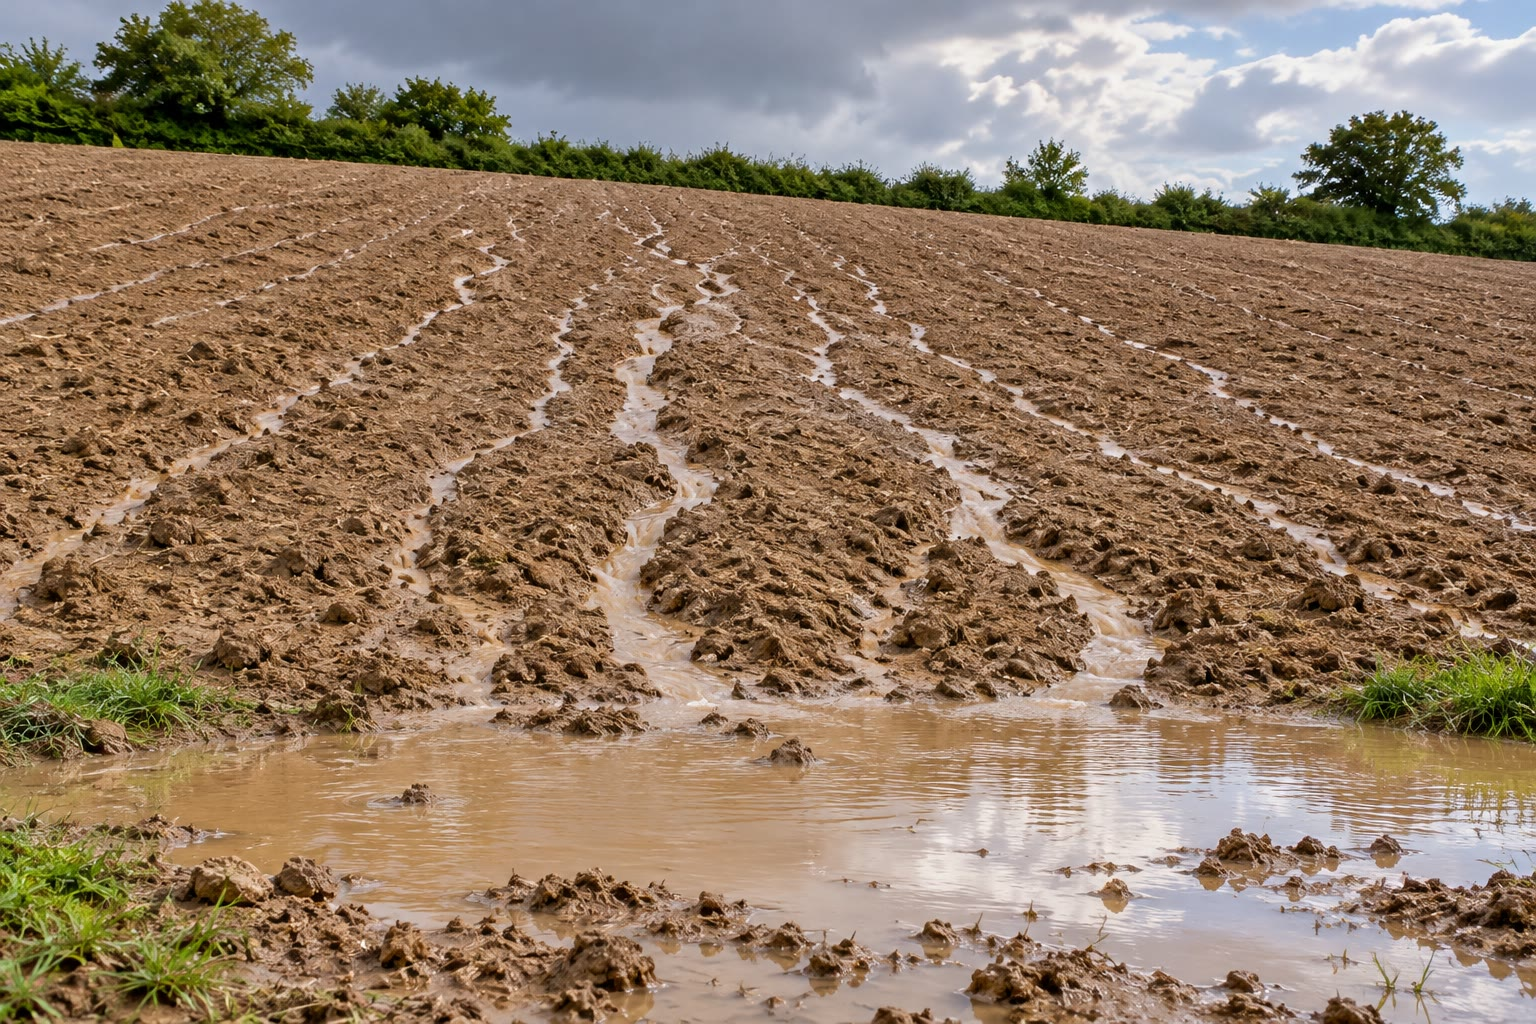
\includegraphics[width=0.72\linewidth]{images/book2/ai/g10-ploughed-rills.jpg}

{\small A ploughed field after a heavy storm: the runoff has cut small
channels, or rills, down the slope and carried the soil into a muddy pool at
its foot.}
\end{omfigure}

\section{Exercises}

\begin{exercise}[$\star$]\label{exo:g10:soil-formation:1}
Define \omterm{def:g10:soil-formation:chemical-weathering}{chemical weathering} and \omterm{def:g10:soil-formation:hydrolysis}{hydrolysis}.
\end{exercise}

\begin{exercise}[$\star$]\label{exo:g10:soil-formation:2}
What is \omterm{def:g10:soil-formation:weathering-profile}{saprolite}? How can you tell \omterm{def:g10:soil-formation:weathering-profile}{saprolite} from a soil formed in sand
brought by a river?
\end{exercise}

\begin{exercise}[$\star$]\label{exo:g10:soil-formation:3}
Name the products of the weathering of a granite: what does each of its
three main minerals become?
\end{exercise}

\begin{exercise}[$\star$]\label{exo:g10:soil-formation:4}
Why are weathered rocks and tropical soils so often red, yellow or brown?
\end{exercise}

\begin{exercise}[$\star$]\label{exo:g10:soil-formation:5}
Using the bar chart, give the median rate of soil production and the median
erosion rate under conventional ploughing. How many times larger is the
second?
\end{exercise}

\begin{exercise}[$\star\star$]\label{exo:g10:soil-formation:6}
Check that the equation of the dissolution of calcite is balanced, for each
element and for the charge.
\end{exercise}

\begin{exercise}[$\star\star$]\label{exo:g10:soil-formation:7}
Limestone dissolves completely, granite leaves sand and clay. Explain the
difference using the two reactions of the chapter.
\end{exercise}

\begin{exercise}[$\star\star$]\label{exo:g10:soil-formation:8}
Explain how the clay--humus complex keeps potassium in a soil that rain
washes through, and how a root takes it.
\end{exercise}

\begin{exercise}[$\star\star$]\label{exo:g10:soil-formation:9}
Give two reasons why \omterm{def:g10:soil-formation:laterite}{laterites} form under hot, wet climates and not under
cold or dry ones.
\end{exercise}

\begin{exercise}[$\star\star$]\label{exo:g10:soil-formation:10}
The median rate of soil production is \qty{0.017}{mm} a year. How long does
it take to form \qty{1}{cm}, \qty{30}{cm} and \qty{1}{m} of soil?
\end{exercise}

\begin{exercise}[$\star\star$]\label{exo:g10:soil-formation:11}
Erosion rates are often given as a mass of soil per hectare per year. With a
soil density of \qty{1200}{kg/m^3}, what mass does a loss of
\qty{1.5}{mm} a year represent on one hectare (\qty{10000}{m^2})?
\end{exercise}

\begin{exercise}[$\star\star\star$]\label{exo:g10:soil-formation:12}
\omterm{def:g10:soil-formation:weathering-profile}{Saprolite} \qty{46}{m} thick has formed under the hills of a temperate region.
If weathering advanced into the rock at \qty{0.017}{mm} a year, how long would
it have taken? What does the answer suggest about the age of such a
landscape?
\end{exercise}

\begin{exercise}[$\star\star\star$]\label{exo:g10:soil-formation:13}
Write the equation of the oxidation of \ce{Fe^2+} into goethite given in the
chapter and check it. Then write and balance the oxidation of \ce{Fe^2+} into
hematite, \ce{Fe2O3}, by oxygen and water, releasing \ce{H+}.
\end{exercise}

\begin{exercise}[$\star\star\star$]\label{exo:g10:soil-formation:14}
Under conservation farming the median erosion rate is \qty{0.082}{mm} a
year. With soil production at \qty{0.017}{mm} a year, how long does it take
to lose \qty{30}{cm} of soil? Compare with conventional ploughing.
\end{exercise}

\begin{exercise}[$\star\star\star$]\label{exo:g10:soil-formation:15}
A granite contains \qty{30}{\percent} orthoclase by mass. What mass of
kaolinite forms when one tonne of this granite has had all its orthoclase
weathered, and what mass of potassium is released?
\end{exercise}

\section{Problem: The Lifetime of a Soil}

\begin{problem}[{Weekend problem --- from rock to field and back to the river}]
\label{pb:g10:soil-formation:1}
% ledger: montgomery:rates, montgomery:lifetime, webmineral:formulas (values computed in figdata/grade-10/soil_rates.py)

\begin{center}
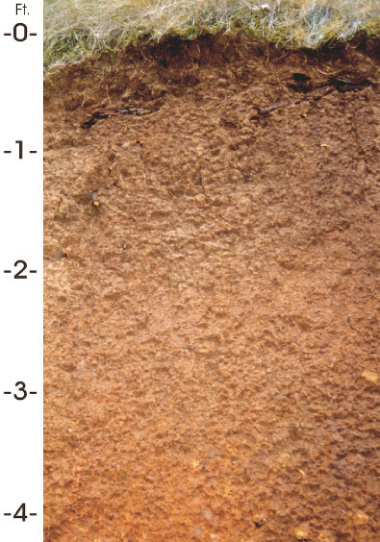
\includegraphics[height=6cm]{images/book2/g10-nrcs-jory-soil.jpg}

{\small A soil profile, with a scale in feet on the left (\num{1}~foot =
\qty{0.3048}{m}). Photograph: USDA Natural Resources Conservation Service
(public domain).}
\end{center}

\medskip
\noindent\textbf{Part I --- A profile.}
\begin{enumerate}
  \item The scale reaches 4 feet near the bottom of the picture. How deep is
        that, in metres?
  \item The dark layer at the top reaches about half a foot. How thick is it,
        in centimetres?
  \item What gives this top layer its dark colour?
  \item Below, the soil is reddish brown. Which minerals give it this
        colour, and how did they form?
  \item Is the \omterm{def:g10:soil-formation:weathering-profile}{parent rock} visible in the photograph? What would you expect
        to find below the bottom of the picture?
\end{enumerate}

\medskip
\noindent\textbf{Part II --- The chemistry of a weathering granite.}
\begin{enumerate}[resume]
  \item Write the equation of the \omterm{def:g10:soil-formation:hydrolysis}{hydrolysis} of orthoclase.
  \item How many moles of orthoclase are there in \qty{1}{kg}
        (\qty{278.33}{g/mol})?
  \item What mass of kaolinite (\qty{258.16}{g/mol}) do they give?
  \item What leaves in the water, and where does it go?
  \item What happens to the quartz of the granite?
\end{enumerate}

\medskip
\noindent\textbf{Part III --- Formation against erosion.}
\begin{enumerate}[resume]
  \item Soil forms at \qty{0.017}{mm} a year. How long does it take to form
        the profile of Part I?
  \item Under conventional ploughing, soil is eroded at \qty{1.537}{mm} a
        year. What is the net loss each year?
  \item How long would the profile of Part I last?
  \item Compare the two times of questions 11 and 13.
  \item Under natural vegetation, erosion is \qty{0.013}{mm} a year. Is the
        soil being lost?
\end{enumerate}

\medskip
\noindent\textbf{Part IV --- The soil's lifetime.}
\begin{enumerate}[resume]
  \item Write the time $T$ to lose a thickness $S$ of soil as a function of
        $S$, of the erosion rate $E$ and of the production rate $P$.
  \item Compute $T$ for $S = \qty{30}{cm}$ under conventional ploughing.
  \item Compute $T$ for $S = \qty{30}{cm}$ under conservation farming
        (\qty{0.082}{mm} a year).
  \item Why can a soil be called a resource that is not renewed on human
        time scales?
  \item How long does it take to lose a metre of soil under conventional
        ploughing?
\end{enumerate}
\end{problem}
